% !Mode:: "TeX:UTF-8"%確保文檔utf-8編碼
\documentclass[tikz,border=2pt]{standalone}
\usepackage{pgfplots}
\usetikzlibrary{calc}
\pgfplotsset{compat=newest}
\begin{document}
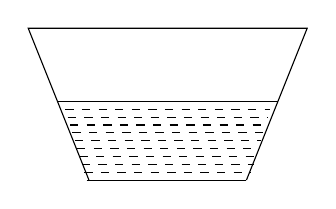
\begin{tikzpicture}
\draw (-1,0) -- (1,0);
\foreach \y [count=\i]  in{0,0.1,...,1}{
\pgfmathsetmacro{\x}{0.03*\i}
\draw[dashed] (-1-\x,\y) -- (1+\x,\y);
}

\draw (-1,0)  -- (-1-0.4,1)-- ($(-1.4,1)!-1cm!(-1,0)$) -- ($(1.4,1)!-1cm!(1,0)$) -- (1,0);
\draw (-1.4,1) -- (1.4,1);


\end{tikzpicture}
\end{document}